\documentclass[12pt]{article}
\usepackage{pdfpages}
\usepackage{dirtytalk}
\usepackage{geometry,graphicx,etoolbox,breakcites,natbib,cite,color,hyperref,enumerate,amsmath,dsfont,lscape,tocloft,booktabs,draftwatermark,times}
\usepackage[export]{adjustbox}
\usepackage[onehalfspacing]{setspace}
\usepackage{hyperref}
\usepackage{csvsimple}
\usepackage{booktabs}
\usepackage{adjustbox}
\usepackage{caption}
\usepackage[bottom]{footmisc}
\usepackage{ragged2e} 
\usepackage{rotating}
\usepackage{natbib}
\usepackage{multirow}
\usepackage{amsmath}
\usepackage{ulem}
\usepackage{titling}
\usepackage[table]{xcolor}
\makeatletter
\patchcmd{\@citex}{,}{;}{}{}
\makeatother
\SetWatermarkText{}\SetWatermarkLightness{0.85} \SetWatermarkScale{4}
\geometry{verbose,lmargin=1in,rmargin=1in, bmargin=1in}
\usepackage[style=apa,backend=biber]{biblatex}
\renewcommand*{\labelnamepunct}{\addcolon\space}
\addbibresource{bibliography.bib}

\begin{document}




\title{Unlocking Potential: The Impact of Savings Groups on Household Welfare Outcomes in Uganda \\ via Staggered Adoption}
\author{Puja Parmar\thanks{Department of Economics, University of Oregon, Eugene, OR 97403-1285, USA, pujap@uoregon.edu.}}
\date{\today}

\sloppy
\maketitle
\doublespacing
\renewcommand{\cftsecleader}{\cftdotfill{\cftdotsep}}
%\tableofcontents

\begin{abstract}
\singlespacing{

Access to financial services plays an important role in economic development, particularly for the under-served populations. In low-income settings they are often shown to improve food security and ability to make lump-sum payments to purchase durable assets, even in situations where there are no improvements in income. In rural areas, means to formal savings are limited and access to savings is often achieved by participating in savings groups which may provide similar benefits. I study the impact of savings groups in the context of Uganda using National Panel Survey data from 2010-2020, during a period of rapid expansion of savings groups. I use a TWFE model that exploits the variation in the timing of arrival of a savings groups in a community. I find that savings groups significantly increase household’s average value of assets by roughly 19\%, however they do not have a significant impact on monthly household earnings. I also observe that savings groups improves the variety of foods consumed by households as well as the expenditure on food consumption. I also validate that bulk quantities do trade at a discount to small quantities which means that households with savings would be less sensitive to price volatility if they made bulk purchases from savings. However, I do not find a significant evidence of increase in bulk purchases of storable foodstuffs due to exposure to savings groups. 
\\
}

\noindent \textbf{JEL classification:} C93, G20, O12, O13, O16, Q12

\noindent \textbf{Keywords:} Keywords: Saving Groups, Village Savings and Loans Associations, Consumption Smoothing, Bulk purchases, Financial Inclusion, SACCOs

\end{abstract} 
\clearpage

\section{Introduction}\label{sec:introduction}

\hspace{1cm} Uganda, a landlocked country in East Africa, while rich in natural resources and cultural diversity, grapples with significant challenges related to poverty, hunger, and financial accessibility, impacting its development. According to the \href{https://www.worldbank.org/en/topic/poverty/publication/poverty-and-equity-briefs}{World Bank}, approximately 21.4\% of the population lives below the national poverty line as of 2020, with rural areas experiencing higher rates of deprivation. Food insecurity remains a pressing issue, with 34\% of Ugandans classified as food insecure, as reported by the \href{https://www.wfp.org/publications/global-report-food-crises-grfc}{Global Network Against Food Crises (2021)}. Access to nutritious food remains a critical issue, as many families struggle with food insecurity, exacerbated by climate change and inconsistent agricultural yields. Financial accessibility is also a major hurdle, as only about 49\% of adults having access to formal financial institutions, as noted by the \href{https://www.ubos.org/wp-content/uploads/publications/09_2021Uganda-National-Survey-Report-2019-2020.pdf}{Uganda Bureau of Statistics (2019)}. The limited banking infrastructure and high interest rates hinder many from obtaining loans or opening and maintaining savings accounts. This combination of factors hinder economic growth and development perpetuating a cycle of deprivation, making it difficult for communities to break free from poverty and improve their living standards.

\hspace{1cm} In recent years, Uganda has witnessed a significant rise in the prominence and impact of savings groups and Village Savings and Loan Associations (VSLAs). These grass-root financial mechanisms have gained remarkable traction in the country's economic landscape due to their potential to enhance financial inclusion, stimulate local economies, and improve livelihoods. Savings groups and VSLAs represent a critical innovation in the realm of financial services, particularly in rural and under-served areas, especially when access to traditional financial services has been limited, with many communities lacking proximity to formal banking institutions. Thus, savings groups and VSLAs have emerged as vital alternatives, offering community-driven solutions to address the gaps in financial accessibility and in encouraging entrepreneurial activities, savings behavior as  well as bringing people out of perpetuated cycles of poverty. Understanding their role and importance is crucial for optimizing the benefits of savings groups and VSLAs and for informed policy interventions aimed at enhancing their efficacy. 

\hspace{1cm}  The primary objective of this paper is to critically analyze the role and impact of savings groups and VSLAs in Uganda, examining their contributions to household welfare as measured by asset ownership and value, earnings, household amenities and food security. Savings groups can act as vehicle of productive investments into assets, improvement in household business outcomes, female empowerment, etc. I am also particularly interested in the mechanism through which savings groups can impact food security. Even without an increase in income, savings groups could impact food security by relaxing liquidity constraints on a household. Households could use loans or savings to take advantage of the arbitrage opportunities in the purchasing of durable storeable foodstuffs. This is because prices of basic foodstuffs have large and predictable seasonal variation and bulk quantities trade at a discount to small quantities.  

\hspace{1cm} Thus purchasing in bulk offers the buyer an income effect from the price discount, moreover bulk purchasing offers an insurance against price volatility. However bulk purchasing requires access to large lump-sum amount of money that can potentially come from savings. Households with savings can purchase in bulk when the prices are low and consume it later, so households can adjust the timing of their expenditure to the season when prices are lower, meaning they can even out the consumption timing from savings. Thus, households without savings would be more exposed to variation in prices whereas households with savings would be less sensitive to price volatility. 


\hspace{1cm} My paper contributes to the growing literature that examines the impact of savings groups on economic outcomes in Uganda and the broader Sub-Saharan African context, focusing on key themes including financial inclusion, economic empowerment, and social outcomes. Previously, impact evaluation studies have demonstrated the role of savings groups in improving food security, overall consumption smoothing, livestock holding, household business outcomes and women’s empowerment, etc. (see {\cite{beaman}, \cite{gash}). These studies are based on randomized control trials of limited duration or they have focused on a very specialized subset of population (see \cite{amponsah}) or a specific purpose of analysis (see \cite{dupas}). To my knowledge my paper is among the first ones to shift to a longer time horizon rich dataset spanning 2010-2020; that replicates some of the previous results from RCTs and uncovers new channels of impact. I also perform \hyperref[sec:robustness]{robustness} checks to ensure that there is no selection in terms of where savings groups get established. I in fact find that NGOs randomly establish savings groups in different communities in Uganda irrespective of the community characteristics; however they do cater to urban areas first before expanding on to rural areas over time. My findings on the role of savings groups in improving household asset ownership is consistent with the results from \cite{bundervoet}. \cite{marguerie} also observe that VSLAs have significant impact on assets but insignificant impact on earnings in their RCT intervention in Côte d’Ivoire. \cite{goldberg} perform a randomized control trial that enhanced financial intermediation by introducing two formal banking products–a savings account and a loan account– to existing savings groups in five districts in Uganda. They find that this linkage intermediation results in a statistically insignificant 13\% increase in self-reported income which is consistent with my findings of regressing conditional monthly household earnings on treatment variable. \cite{seep} in their report compile results from 53 studies that assess the role of savings groups on different economic and social outcomes. The report also validates that a fair amount of evidence exists supporting that savings groups participation leads to an increase in asset ownership; while they also found a mixed evidence on consumption and food expenditure. The report also confirms that there is only a small evidence that savings groups lead to an increase in income, as also a small evidence that savings groups increase business ownership. Finally, the report also supports my findings on improvements in food variety consumed and increase in food expenditures as a result of exposure to savings groups. \cite{frisancho} on the other hand observe an insignificant effect on household assets but significant improvements in roof quality in rural Peru using a cluster randomized control trial. My results are also consistent with the fact that the literature on saving groups rarely reports improvements in business outcomes like business expansion or increase in entrepreneurial activities (\cite{beaman}, \cite{ksoll}), with the notable exception of \cite{karlan}.


\hspace{1cm} My paper also contributes in the literature of assessing impact of savings groups on outcomes other than household income and assets; for instance household amenities. Using a cluster randomized trial, \cite{ksoll} investigate the impact of VSLAs in Northern Malawi over a two year period and find evidence of positive and significant intention-to-treat effects on several outcomes, including the number of meals consumed per day, household expenditure, and the number of rooms in the dwelling. In this paper, I extend the analysis to look at additional outcomes like quality of roof, access to electricity, own toilets and own water source, improved walls and floor quality of houses and assess if savings groups have any positive impact on those outcomes.  

\hspace{1cm}
 \cite{karlan} in their paper using a clustered randomized evaluation spanning three African countries (Ghana, Malawi, and Uganda), find that the promotion of community-based microfinance groups leads to an improvement in household business outcomes and women’s empowerment. However,
they do not find evidence of impacts on average consumption or other livelihoods. My paper looks at similar measures albeit only for Uganda over a larger time horizon.

\hspace{1cm} While most of the theoretical models on commodity storage are developed in a developing country’s context, there are only a few empirical studies that investigate household grain storage decisions in Sub-Saharan Africa. My paper relates to the literature on strategic holding of bulk food items. \cite{tesfaye} shed light on maize storage behavior and investigate the effect of climatic factors, improved storage practices, and household characteristics on grain storage behavior. They attribute grain storage practice in Ethiopian households to factors like crop protection technology, rainfall shocks, temperature and health shocks among other things. My paper on the other hand studies the channel of savings groups as a contributor to bulk purchasing behavior in Ugandan households. \cite{aggarwal} in their paper used a novel approach where they encouraged randomly selected ROSCAs to set aside maize together in communal bags, stored at a single member's house (usually the ROSCA treasurer) in Kenya. They provided ROSCAs with storage supplies, namely triple-layered plastic bags capable of being hermetically sealed and designed specifically for the purpose of grain storage, and a heavily subsidized wooden stand to keep the maize elevated from the ground (and less susceptible to pests and water damage). They found that this technique increased storage among smallholder farmers providing savings clubs with a simple way to set aside maize for storage.

\hspace{1cm} I also build on the literature studying role of savings in improving food security by virtue of greater diversity of foods consumed, improved food security and increased food expenditure/consumption (\cite{bass}, \cite{Kiiza}, \cite{beaman}) find that savings groups have a positive and significant impact on household dietary diversity score, food consumption score, and food expenditure. 

\hspace{1cm} The rest of the paper is organized as follows. Section 2 provides a background on savings groups while section 3 provides information on the data used for analysis in this paper. I discuss thoroughly the methodology in the next section followed by results from regression analysis. I study the mechanism of bulk purchases explicitly in the next section followed by results corresponding to the same. I extend the results from hetereogeneity analysis in section 6  and perform robustness checks in section 7. I finally conclude my paper in section 8.


\section{Background on Savings Groups}\label{sec:background}
\hspace{1cm} Savings groups are community-based financial institutions which typically consist of small, self-managed assemblies of individuals who pool their resources to provide mutual financial support. They are generally comprised of 20 to 30 members, who meet weekly over the operating cycle (typically lasting one year). At the end of the cycle all funds are shared among the group’s members in  proportion to the amount saved during the period of operation. Members of an savings groups pool savings within the group, borrow from the group at an interest, and receive a return on their savings. Each week, members contribute funds to the group, repay previous loans, and request new loans. Hence, a member who wishes to borrow must first save. Funds that are not lent out are stored in a safe and can be lent out in the future. Finally, at the end of the operating cycle of the group, all loans are repaid and each member receives back the amount saved with the group, plus a return on her savings that depends on the total interest payment collected by the group. After the share out, the composition of the group may change, and a new cycle may start.

\hspace{1cm} Thus, savings groups facilitate financial flows within local communities, and have received a lot of attention from policy makers in the past decade. Because they can be set up and maintained with minimal outside intervention, savings groups have spread very fast in sub-Saharan Africa and other developing countries. Savings groups are an innovative instrument for bringing financial inclusion to ultra-poor, vulnerable households who are usually not reached by traditional banking or microfinance interventions. For instance, the Gates Foundation has provided significant resources to Catholic Relief Services, CARE International, and Oxfam to develop such groups in
sub-Saharan Africa\footnote{See \url{https://docs.gatesfoundation.org/Documents/one-early-success-story.pdf.}} Consequently, membership in savings groups reached 10.5 millions people worldwide in 2014, a tenfold increase relative to 2008, and continues to climb (\cite{burlando}). In Fig. \ref{fig:fig1}, we can see a rapid expansion in the parishes exposed to savings groups from 51\% in 2010 to 86\% by 2019-20 in Uganda. By facilitating access to credit and encouraging saving habits, savings groups and VSLAs contribute to increased household resilience, improved business opportunities, and enhanced community cohesion. In Uganda, the formalization of savings groups began in the 1990s, with support from NGOs and development agencies. In this paper, I empirically study how the timing of entry of savings groups in a community affects the consumption behavior and welfare of community members.

\graphicspath{{Images/}}
\begin{figure}[ht]
\makebox[\textwidth][c]{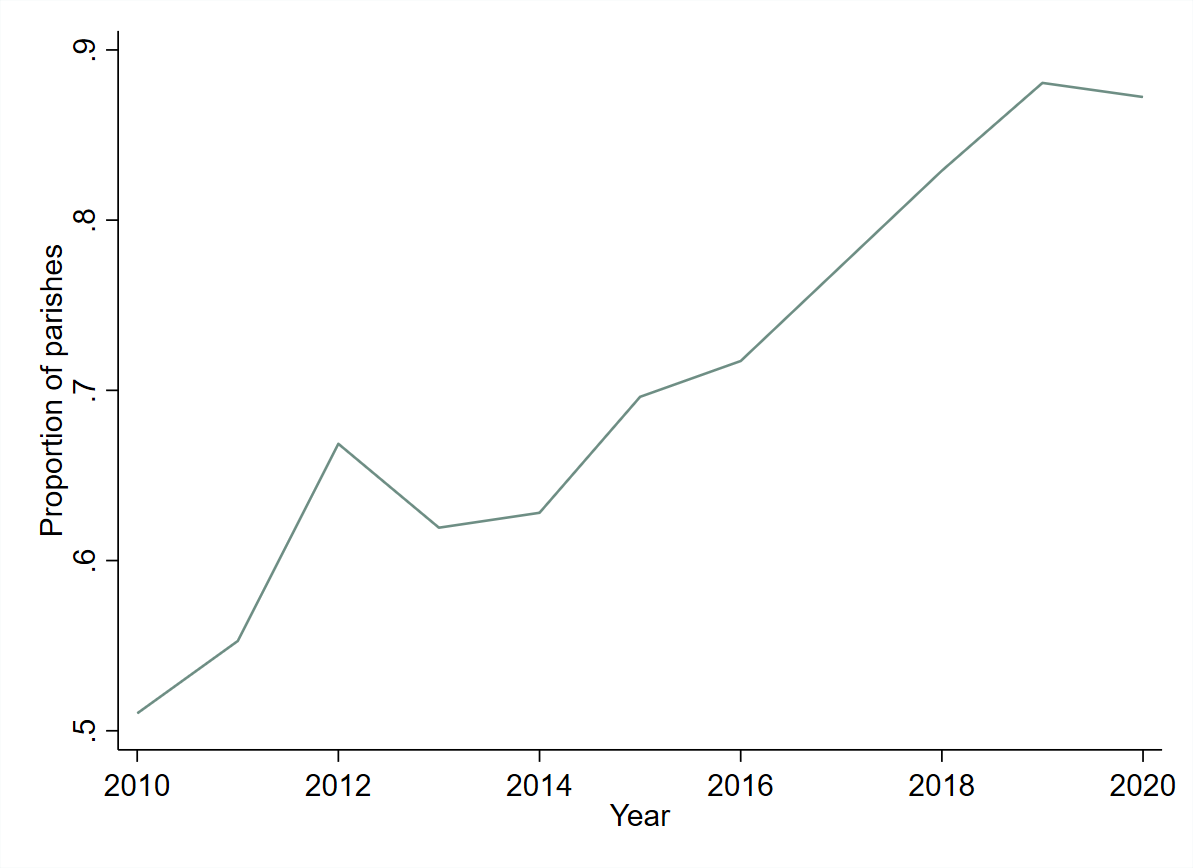
\includegraphics[frame,width=18cm, height=15cm]{parish_exposure_graph.png}}
\caption{\textbf{Expansion of savings group in local parish over year of survey in Uganda}}
\label{fig:fig1}
\footnotesize{\textbf{(Notes: }The graph shows proportion of parishes that are treated i.e. exposed to at least 1 savings group by year of interview. There was quite a bit of parish restructuring that happened across our panel survey years. This means that we have certain parishes which didn't follow through in community module post 2011-12. Also, a lot of new parishes started emerging in community module since 2013-14 for which earlier community data is not available. Thus, I do not have a consistent baseline of parishes to track the growth of savings groups exposure. However, I do have the quantitative information to make comparisons. To elaborate this further, I have 224 unique parishes in wave 2 out of which 110 were exposed to savings groups. On the other hand I have 465 parishes in wave 7 out of which 402 were exposed to savings groups. This demonstrates that expansion of savings groups has in fact be significant, since we have more total number of parishes in the most recent wave and also more significant chunk of those parishes as being exposed to savings groups.}
\end{figure}
\clearpage



\section{Data}\label{sec:2.a Data} 
\hspace{1cm} For the purpose of this study, I will be using data from Uganda National Panel Survey from 2010-2020. The UNPS is carried out annually, over a twelve-month period on a nationally representative sample of households, for the purpose of accommodating the seasonality associated with the composition of and expenditures on consumption. The survey is conducted in two visits in order to better capture agricultural outcomes associated with the two cropping seasons of the country. The UNPS has been set out to track and re-interview 3,123 households that were distributed over 322 enumeration areas (EAs), selected out of the 783 EAs that had been visited by the Uganda National Household Survey (UNHS) in 2005-06. The UNPS aims at producing annual estimates in key policy areas and at providing a platform for experimenting with and assessing of national policies and programs. 

\hspace{1cm} I gather information on household demographics (see \hyperref[sec:appendix]{Appendix}), monthly earnings, asset ownership and value as well as household amenities from the household module. I fetch information on all products consumed by the household in the last 7 days including their market prices and units of purchase from the consumption module. I delve into the community module to gather information on presence and characteristics of savings groups in the communities in which the households belong. These characteristics include information on group beginning year, number of female members in the group and frequency of group
meetings. Lastly, I also use the GDP deflator linked series and Official Exchange Rate data from World Bank to convert household (HH) assets and earnings in terms of inflation-adjusted US dollars. It is to be noted that the UNPS survey revised the manner in which the unique HH - ID key was designed multiple times across years - this is important for us since we want to track the households right from 2010-11 until 2019-20 which means we need to have consistent HH - ID keys to panelize them. I have listed the detailed process I use to get consistent household IDs across years in \hyperref[sec:appendix]{Appendix}.

\hspace{1cm} The dataset contains approximately 100 consumption items at the raw level - which I standardize and bring down to 11 consumption items which are non-perishable (durable) in nature and therefore can be purchased in bulk. The detailed description can be found in \hyperref[sec:appendix]{Appendix}. Similarly, the dataset has many non-standardized unit codes which I convert in terms of kilograms / liters as standards of unit. Since Matooke is one of the most important dietary items of consumption, I describe the methodology of converting Matooke units of consumption to standardized units in \hyperref[sec:appendix]{Appendix}. 

\hspace{1cm} The community section module collects information on whether a savings group exists in a particular parish or not. The survey collects information on group beginning year, total number of groups in the community, number of female members in the group, frequency of group meetings, etc. Even though I cannot link directly household's participation into savings groups, I proxy it by parish exposure. I obtain parish level information on the savings groups and construct measures for timing of entry of savings groups into a parish. I then link all the households that correspond to these parishes with the savings groups information. I describe the detailed process of linking community survey with household survey in \hyperref[sec:appendix]{Appendix}. In other words if a household belongs to a parish that got introduced to savings groups, I mark the household as `treated' thereon. Thus, savings groups affects households by virtue of their timing of entry into a given parish.

\hspace{1cm} Note that the community section collects data on a limited sample of parishes, hence for households belonging to any parish outside of this scope, I have to drop the households as they do not have any corresponding savings group information. This leaves me with roughly 400 parishes that can be linked between household and community modules and that can offer information on savings groups. In this way I retain survey data on monthly earnings, value of assets owned, primary occupation as well as other household and demographic characteristics like sex of household head, marital status, educational level, age composition of members, etc. and their corresponding community module information for 3670 unique households. 

\hspace{1cm} Since all households do not consume all the available products, I have an unbalanced panel when it comes to the products consumed. Hence, I balance out my panel by adding extra rows for each household - one for each of the product not consumed by the household in a given year. Then I populate all the remaining household and community particulars except for the consumption and pricing related information which are left missing for the products not consumed. After all of the data cleaning operations performed so far, I recheck if there are any households that appear just a single year data and therefore cannot be panelized and I drop all such households. This leaves me with 2756 unique households that repeat across years. 

\hspace{1cm} In the final step of data cleaning I create a new dummy variable which takes the value of 1 if the product is perishable and 0 otherwise. After dropping all those commodities which have a share of less than 1\% in the total value consumed by household as well as dropping the commodities which cannot be purchased in bulk (that is the perishables) I am left with household-demographic-product-community information for 2753 unique households, which I use for my regression analyses.

\subsection{Summary statistics}\label{sec:summary statistics}
\hspace{1cm} Table \ref{table:summary statistics} reports the summary statistics of the key variables of interest. Over the period of 2010-2020, the sampled households have on average a monthly earnings of (\$61). In order to prevent extreme value outliers in data I have winsorized 5\% of the data from top and bottom which gives me an average monthly earnings of \$27. Similarly, I observe an yearly ownership of assets worth \$5031 which come down to \$2659 after winsorization. Savings group have expanded to most of the parishes with an average of 74.7\% expansion rate out of all the parishes in our sample. Out of the total purchases made by households for consumption purposes, 15.5\% account for purchases in bulk.

\hspace{1cm} Comparing the household characteristics shows us that roughly 33\% of the households are female headed. Most of the household heads report to be married and have at least some level of positive schooling. Only about 23\% of the households live in urban areas, and most of the household members belong in the age group 16-59 years. Almost 19\% of the households report to be poor on average. Finally, approximately 38\% of the households have some kind of business, 72\% have at at least 1 member owning a mobile phone and almost 83\% of the households have at least 1 member who has at least some form of savings. 

\hspace{1cm} The household composition is such that on average we have 1.6 members in the age group of 6-15 years, 2.25 members in the age group of 16-59 years and 0.33 members in the age group of 60 and above. The households live in a dwelling comprising of 0.57 rooms per capita on average, with 13.4\% of the households having access to electricity while 19\% of the households have ownership of some land. Almost 34\% of the households have their own private toilet and around 32\% have own source of water; while 71\% of the households report having improved roof quality (non-mud, non-thatch roofs), 33\% report improved floor materials and 44\% report improved materials used for external wall construction. Next I also break down the dietary patterns of the households in the last 7 days into 11 different categories of consumption - on average I observe that households consume at least 8 different categories of food. They also report an average food expenditure of 21\$. Finally, I observe that almost 41\% of the households have faced some kind of shock.


\begin{table}[!h]
\centering
\begin{tabular}{llllll}
\hline
    & \multicolumn{6} {c|} {\bfseries Variable} & {\bfseries  Mean}  & {\bfseries Min} & {\bfseries Max}  & {\bfseries No. of Obs} & \\
\cline{1-5}
\multicolumn{1}{|r}{Monthly HH earnings deflated (in \$)} &
  \multicolumn{1}{|r}{61.352} &
  \multicolumn{1}{|r}{0} &
  \multicolumn{1}{|r}{1,77,256} &
  \multicolumn{1}{|r|}{9,629} \\
\multicolumn{1}{|r}{Monthly HH earnings deflated (in \$), 5\%} &
  \multicolumn{1}{|r}{27.128} &
  \multicolumn{1}{|r}{0} &
  \multicolumn{1}{|r}{188.220} &
  \multicolumn{1}{|r|}{9,629}  \\
\multicolumn{1}{|r}{Total value of assets deflated (in \$)} &
  \multicolumn{1}{|r}{5,031} &
  \multicolumn{1}{|r}{0} &
  \multicolumn{1}{|r}{1,671,263} &
  \multicolumn{1}{|r|}{9,614}  \\
\multicolumn{1}{|r|}{Total value of assets deflated (in \$), 5\%w} &
  \multicolumn{1}{|r}{2,659} &
  \multicolumn{1}{|r}{45.173} &
  \multicolumn{1}{|r}{18,313} &
  \multicolumn{1}{|r|}{9,614}  \\
\multicolumn{1}{|r}{SavingsGroups in parish} &
  \multicolumn{1}{|r}{0.747} &
  \multicolumn{1}{|r}{0} &
  \multicolumn{1}{|r}{1} &
  \multicolumn{1}{|r|}{9,629}  \\
\multicolumn{1}{|r}{HH head is female} &
  \multicolumn{1}{|r}{0.335} &
  \multicolumn{1}{|r}{0} &
  \multicolumn{1}{|r}{1} &
  \multicolumn{1}{|r|}{9,629}  \\
\multicolumn{1}{|r}{HH head is married} &
  \multicolumn{1}{|r}{0.721} &
  \multicolumn{1}{|r}{0} &
  \multicolumn{1}{|r}{1} &
  \multicolumn{1}{|r|}{9,629}  \\
\multicolumn{1}{|r}{HH is urban} &
  \multicolumn{1}{|r}{0.229} &
  \multicolumn{1}{|r}{0} &
  \multicolumn{1}{|r}{1} &
  \multicolumn{1}{|r|}{9,629}\\
\multicolumn{1}{|r}{HH head has some schooling} &
  \multicolumn{1}{|r}{0.846} &
  \multicolumn{1}{|r}{0} &
  \multicolumn{1}{|r}{1} &
  \multicolumn{1}{|r|}{9,629}  \\
\multicolumn{1}{|r}{No. of members (6-15 yrs)} &
  \multicolumn{1}{|r}{1.605} &
  \multicolumn{1}{|r}{0} &
  \multicolumn{1}{|r}{11} &
  \multicolumn{1}{|r|}{9,629}  \\
\multicolumn{1}{|r}{No. of members (16-59 yrs)} &
  \multicolumn{1}{|r}{2.252} &
  \multicolumn{1}{|r}{0} &
  \multicolumn{1}{|r}{12} &
  \multicolumn{1}{|r|}{9,629}  \\
\multicolumn{1}{|r}{No. of members (60 yrs or above)} &
  \multicolumn{1}{|r}{0.329} &
  \multicolumn{1}{|r}{0} &
  \multicolumn{1}{|r}{4} &
  \multicolumn{1}{|r|}{9,629}  \\
\multicolumn{1}{|r}{HH is poor} &
  \multicolumn{1}{|r}{0.194} &
  \multicolumn{1}{|r}{0} &
  \multicolumn{1}{|r}{1} &
  \multicolumn{1}{|r|}{9,629}  \\
\multicolumn{1}{|r}{HH with current earnings} &
  \multicolumn{1}{|r}{0.295} &
  \multicolumn{1}{|r}{0} &
  \multicolumn{1}{|r}{1} &
  \multicolumn{1}{|r|}{9,629}  \\
\multicolumn{1}{|r}{HH-Business dummy} &
  \multicolumn{1}{|r}{0.378} &
  \multicolumn{1}{|r}{0} &
  \multicolumn{1}{|r}{1} &
  \multicolumn{1}{|r|}{9,629} \\
\multicolumn{1}{|r}{Mobile ownership dummy} &
  \multicolumn{1}{|r}{0.717} &
  \multicolumn{1}{|r}{0} &
  \multicolumn{1}{|r}{1} &
  \multicolumn{1}{|r|}{9,613}  \\
\multicolumn{1}{|r}{Savings dummy} &
  \multicolumn{1}{|r}{0.831} &
  \multicolumn{1}{|r}{0} &
  \multicolumn{1}{|r}{1} &
  \multicolumn{1}{|r|}{4,415}  \\
\multicolumn{1}{|r}{Number of rooms per capita} &
  \multicolumn{1}{|r}{0.571} &
  \multicolumn{1}{|r}{0.111} &
  \multicolumn{1}{|r}{3} &
  \multicolumn{1}{|r|}{9,583} \\
\multicolumn{1}{|r}{Access to Electricity} &
  \multicolumn{1}{|r}{0.134} &
  \multicolumn{1}{|r}{0} &
  \multicolumn{1}{|r}{1} &
  \multicolumn{1}{|r|}{9,616}  \\
\multicolumn{1}{|r}{Ownership of Land} &
  \multicolumn{1}{|r}{0.188} &
  \multicolumn{1}{|r}{0} &
  \multicolumn{1}{|r}{1} &
  \multicolumn{1}{|r|}{9,613} \\
\multicolumn{1}{|r}{Access to own toilet} &
  \multicolumn{1}{|r}{0.340} &
  \multicolumn{1}{|r}{0} &
  \multicolumn{1}{|r}{1} &
  \multicolumn{1}{|r|}{9,614} \\
\multicolumn{1}{|r}{Access to own water source} &
  \multicolumn{1}{|r}{0.322} &
  \multicolumn{1}{|r}{0} &
  \multicolumn{1}{|r}{1} &
  \multicolumn{1}{|r|}{9,614} \\
\multicolumn{1}{|r}{Improved roof} &
  \multicolumn{1}{|r}{0.707} &
  \multicolumn{1}{|r}{0} &
  \multicolumn{1}{|r}{1} &
  \multicolumn{1}{|r|}{9,616} \\
\multicolumn{1}{|r}{Improved floor} &
  \multicolumn{1}{|r}{0.331} &
  \multicolumn{1}{|r}{0} &
  \multicolumn{1}{|r}{1} &
  \multicolumn{1}{|r|}{9,614} \\
\multicolumn{1}{|r}{Improved wall} &
  \multicolumn{1}{|r}{0.439} &
  \multicolumn{1}{|r}{0} &
  \multicolumn{1}{|r}{1} &
  \multicolumn{1}{|r|}{9,614} \\
\multicolumn{1}{|r}{Amenities Index} &
  \multicolumn{1}{|r}{0} &
  \multicolumn{1}{|r}{-1.442} &
  \multicolumn{1}{|r}{3.501} &
  \multicolumn{1}{|r|}{9,616} \\
\multicolumn{1}{|r}{Food variety index} &
  \multicolumn{1}{|r}{8.208} &
  \multicolumn{1}{|r}{1} &
  \multicolumn{1}{|r}{11} &
  \multicolumn{1}{|r|}{9,446} \\
\multicolumn{1}{|r}{Food expenditure (in deflated \$)} &
  \multicolumn{1}{|r}{20.835} &
  \multicolumn{1}{|r}{0.943} &
  \multicolumn{1}{|r}{1,039.548} &
  \multicolumn{1}{|r|}{9,446} \\
\multicolumn{1}{|r}{Any shock dummy} &
  \multicolumn{1}{|r}{0.408} &
  \multicolumn{1}{|r}{0} &
  \multicolumn{1}{|r}{1} &
  \multicolumn{1}{|r|}{8,167}\\
\multicolumn{1}{|r}{Food index} &
  \multicolumn{1}{|r}{0} &
  \multicolumn{1}{|r}{-2.693} &
  \multicolumn{1}{|r}{33.220} &
  \multicolumn{1}{|r|}{9,446}\\
\multicolumn{1}{|r}{Log price (per kg)} &
  \multicolumn{1}{|r}{6.774} &
  \multicolumn{1}{|r}{0} &
  \multicolumn{1}{|r}{12.024} &
  \multicolumn{1}{|r|}{49,542} \\
\multicolumn{1}{|r}{Bulk purchase dummy - Full} &
  \multicolumn{1}{|r}{0.156} &
  \multicolumn{1}{|r}{0} &
  \multicolumn{1}{|r}{1} &
  \multicolumn{1}{|r|}{105,913}  \\
\cline{1-5}
\end{tabular}
\caption{\bfseries Summary Statistics}
\label{table:summary statistics}
\end{table}


\clearpage

\section{Methodology}\label{sec:Methodology} 
\hspace{1cm} In this paper, I hypothesize that savings groups improve household welfare by increasing household’s assets and earnings, improving household amenities and enhancing food security. In order to test these hypotheses individually, I structure the model as follows: 

\boldmath
\begin{equation}
y_{hpt} = \beta SavingsGroups_{pt}\\
  + f_h + f_p + f_t   + \delta X_{hpt} + \epsilon_{hpt}\\
\end{equation}
\unboldmath

where: \\

\hspace{1cm} 1. Household h is observed over t $>$ 1 years (it’s a panel).

\hspace{1cm} 2. Household h is interviewed at different times of the year across different years.

\hspace{1cm} 3. $y$ stands for outcome variables like total value of household assets, ownership of land dummy, total monthly household earnings, food index, household amenities, etc. 

\hspace{1cm} 4. $f_t$ is the year-month fixed effect. It captures the fact that aggregate household consumption may be seasonal. The time fixed effects control for factors changing each year that are common
to all households and parishes for a given year.

\hspace{1cm} 5. $f_p$ is the parish fixed effect. It captures the group level at which our treatment is happening. It estimates the common difference (to all years) in the outcome variable in parish p relative parish 1, controlling for household characteristics and time-specific characteristics common to all parishes. It is called parish fixed effect precisely because the difference is common to all year-months in parish p; in other words, the `effect' of parish p is `fixed' across all year-months, the parish fixed effects control for baseline differences between parishes.

\hspace{1cm} 6.  $f_h$ is the household fixed effect. It captures the household level preferences which may change across years.

\hspace{1cm} 7. $X_{hpt}$ includes demographic variables like sex of household head, marital status, educational status of household head, number of household members belonging to different age categories in panel. To the extent that composition changes (say, kids age out and eat more) it can influence the decision to buy certain foods. Note that X contains both time-variant as well as time-invariant characteristics. The time-invariant characteristics will automatically drop when we incorporate household fixed effects.

\hspace{1cm} The treatment variable of interest is \textit{`SavingsGroups'} dummy which takes the value of 1 from the time that it is reported when there is at least 1 savings group in parish and 0 otherwise. All households belonging to a given parish will experience the same treatment. Since different parishes can be exposed to savings groups in different time periods we have a staggered adoption of treatment. $\beta$ measures the change in outcome variable due to the treatment \textit {`SavingsGroups'} in a parish. I use the variation in timing of entry of savings groups in a community parish to identify the effect on household assets, earnings, amenities, food security and bulk purchases based on when the community parish reports entry of at least 1 savings group in it, controlling for household characteristics. The first regression in column 1 controls for time fixed effects, parish level fixed effects and household controls. Column 2 includes household fixed effects to account for within household changes across time. The standard errors are clustered at the parish level. 

\hspace{1cm} An additional point to consider is that sometimes savings groups could enter a parish but for a variety of reasons, they may stop operating in between in any given year - this means in a given parish once a savings group has entered it could become inoperative either temporarily or permanently. However, in my paper I do not account for this switch on and switch off of savings groups, rather I only look at the time of entry of the savings groups in a parish and then hold the treatment dummy to be 1 for all years subsequently. Thus our estimates can be interpreted as "intent to treat". In order to find the actual magnitude of treatment effect, I divide the co-efficient estimates with the imputed average membership to savings group. The imputed average membership (IAM) is calculated as number of savings groups in parish times 25 divided by number of households in parish. I then compute the average membership across all parishes across all years which gives me an average value of 0.316. This means that on average for any parish in any year we have 31.6\% of the population participating in savings groups. I report the magnitude of treatment effect along with the intent-to-treat estimates in my regression results in the following subsection.

\subsection{Results from regression analysis}\label{sec:regression1}

\subsection*{Household Assets and Amenities}\label{sec:assets amenities}

\hspace{1cm} For the first set of analysis, I regress the total value of household assets on the treatment variable. I find that wealth in the form of total value of assets owned by households is strongly associated with our treatment of savings group exposure to parish increasing total value of assets by \$519.3 dollars which is 19.5\% of average value of assets owned by households. This gives me an actual magnitude of treatment effect on household assets worth \$1,643.33, which may seem large but it is plausible considering that treatment to savings groups often has a spillover effect in the community thereby benefiting even non-participants to savings groups. 

\hspace{1cm} If I just look at the ownership of land then exposure to savings groups causes a 7\% increase in ownership of land which is statistically insignificant. However, this makes sense since access to land is harder on just savings groups revenues. I also do not find any significant effect on household amenities - this could be due to a number of reasons. For instance, external shocks or even competing priorities like health and education could disrupt savings making it difficult to invest in amenities. Similarly, lack of basic infrastructure like electricity cannot entirely be controlled or influenced by community savings.

\begin{table}[!h]
\centering
\begin{tabular}{lllllll}
 \\
  & \multicolumn{2}{c}{\bfseries  Total HH value of assets} &  \multicolumn{2}{c}{\bfseries  Ownership of land}  &  \multicolumn{2}{c}{\bfseries  Amenities Index} \\
 \cline{1-7}
{\bfseries Variables} & (1) & (2) & (1) & (2) & (1) & (2) \\
\hline
SavingsGroups  & 399.556*	& 519.293***	& 0.017	& 0.013	& -0.047	& -0.024 \\
& (206.704)	& (194.194)	& (0.024)	& (0.024)	&(0.031)	& (0.028) \\
 &  \\
Observations & 9,612	& 9,602 &	9,611	& 9,600	& 9,614	& 9,604 \\
R-squared &	0.382	& 0.768	& 0.347	& 0.563	& 0.623	& 0.885
 \\
Mean of Outcome & 2659.310	& 2659.310	& 0.188	& 0.188	& -0.000 &	-0.000
&
Time F.E. & YES & YES & YES & YES & YES & YES \\
HH Controls & YES & YES & YES & YES & YES & YES \\
Parish F.E. & YES & YES & YES & YES & YES & YES \\
 HH F.E. & NO & YES & NO  & YES & NO  & YES \\ \hline
\cline{1-7}
\end{tabular}
\captionsetup{justification=centering}
\caption{\bfseries Fixed-Effects regression of total value of assets, amenities index and \\ ownership of land on treatment} \\
\label{table:assets and amenities}
\footnotesize{(Notes for table: Outcome variable total household (HH) value of assets is derived by first aggregating the total value of all the assets owned by a household in a given period. Then they are deflated to 2017 prices and finally converted to US dollars using Official Exchange rates. In order to avoid extreme outliers I winsorize 5\% of the distribution on either sides. For Amenities Index, I create a standard normal variable by combining factors like number of rooms per capita, access to electricity, access to own water source and own toilets and roof quality, floor quality and wall quality. Outcome variable ownership of land dummy is a dummy variable that takes the value of 1 if in a given time period, the household reports land as one of the assets owned by household and 0 otherwise. Column 1 represents regression with time and parish fixed effects, column 2 includes household fixed effects as well. The HH controls includes variables like sex of HH head, marital status and educational status of HH head, age composition brackets for household members, etc. Standard errors are clustered at the parish level in parentheses\\
*** p $<$ 0.01, ** p $<$ 0.05, * p $<$ 0.1)} \\
\end{table}


\subsection*{Household Earnings and business}\label{sec:regression earnings}

\hspace{1cm} Next I regress household monthly earnings on the treatment variable. I do three separate set of regressions here - in the full sample I regress on the full sample of households; in the all earners only regression I only take households that report some positive monthly earnings. Finally, in the wage earners only regression, I further reduce my sample by taking only those households that report positive wage earnings. Exposure to savings groups does not seem to have any significant effect on monthly earnings of households in either case. It's important to note that almost half of the sample reports subsistence farming as their most important source of earning - this means we do not have a corresponding measure of HH earnings for most of these households. Thus it's hard to accurately track the impact of savings groups on household's income due to our data limitations. I also regress household business dummy on treatment and find negative significant results at 5\% level.

\begin{table}[!h]
\centering
\begin{tabular}{lllllllll}
 \\
& \multicolumn{2}{c}{\bfseries  All HH} &  \multicolumn{2}{c}{\bfseries  All earners only} &  \multicolumn{2}{c}{\bfseries  Wage earners only} & \multicolumn{2}{c}{\bfseries  HH having business}  \\
\cline{1-9}
 {\bfseries Variables} & (1) & (2)  & (1) & (2) & (1) & (2)   & (1) & (2)   \\
 \hline
SavingsGroups  & 0.426	& 0.704	& 0.555 &	8.993	& 2.134	& 1.871 & -0.045*	& -0.057** \\
& (2.411)	& (2.320) &	(6.301)	& (6.717)	& (8.988)	& (11.272) & (0.026)	& (0.026)\\
 &  \\
Observations & 9,628 &	9,618 & 2,815 &	2,121 &	1,390	& 1,033 & 9,628	& 9,618	 \\
R-squared & 0.276 &	0.662 &	0.408	& 0.752	& 0.544	& 0.821 & 	0.184 &	0.603 \\
Mean of Outcome & 27.128 &	27.128	& 91.946 &	91.946	& 108.243	& 108.243 & 0.378 & 0.378
&
Time F.E.  & YES & YES & YES & YES & YES & YES & YES & YES \\
HH Controls  & YES & YES & YES & YES & YES & YES & YES & YES \\
Parish F.E.  & YES & YES & YES & YES  & YES & YES & YES & YES \\
HH F.E. & NO  & YES  & NO & YES & NO & YES & NO & YES \\ \hline
\cline{1-9}
\end{tabular}
\captionsetup{justification=centering}
\caption{\bfseries Fixed-Effects regression of total household monthly earnings and \\  business dummy on treatment variable}
\label{table: earnings and business}
\footnotesize{(Notes for table: Outcome variable total household (HH) monthly earnings is derived by first aggregating the total monthly earnings of each household member across jobs, and then summing up the monthly earnings for all the members in the household that report to be working. Then they are deflated to 2017 prices and finally converted to US dollars using Official Exchange rates. In order to avoid extreme outliers I winsorize 5\% of the distribution on either sides. I extract two sub-samples of households - one that reports at least some positive earnings and other reports at least some positive wage earnings only. Outcome variable household (HH) having business is derived by looking at if a household member ran a business in the last 12 months and then aggregating it for all household members; if at least one household member reports running a business in the last 12 months then the household business dummy will take the value of 1. Column 1 represents regression with time and parish fixed effects, column 2 includes household fixed effects as well. The HH controls includes variables like sex of HH head, marital status and educational status of HH head, age composition brackets for household members, etc. Standard errors are clustered at the parish level in parentheses\\
*** p $<$ 0.01, ** p $<$ 0.05, * p $<$ 0.1)} 
\end{table}


\pagebreak
\clearpage

\subsection*{Food diversity and expenditures}\label{sec:regression food}

\hspace{1cm} I next delve deeper into the consumption and food security aspects in this section. As mentioned earlier, I breakdown the household consumption in last 7 days into 11 different consumption categories. I individually regress each of the consumption category on the treatment variable and also regress the collective food variety index on treatment. The food variety index can take any value ranging from 0 to 11 depending on how many categories of food the household consumes. It is reasonable to believe that the more diverse consumption patterns a household has, the better the household ranks in terms of nutrition and food security. Finally, I also compute the total value of each goods consumed by each household in a given time period and aggregate it to get the expenditure on food which I deflate to 2017 prices and convert to US dollars. I regress this on the treatment variable to see if exposure to savings groups results in households spending more money on food. I then combine both food variety index and food expenditure into a single standard normal variable which I call the Food Index. Simply put, higher the value on Food Index, better the household is doing in terms of more and better food consumption.

\hspace{1cm} It is important to note that households are prone to a variety of shocks in any given year. The shocks can take any form like irregular rains, theft, death of income earner or serious illness or even unusually high level of crop diseases and pests. On average, 40\% of the households report facing at least one shock in the last year. Thus it is important to look at how households' exposure to shock affects their food consumption and if being exposed to savings groups helps in their food security or not. Thus I run 3 separate set of regressions for food index. Specifically, I first regress both the variables on full set of households. Then, I also regress both the variables on only those sample of households that faced any shock in the previous year and on only those sample of households that did not face any shock in the previous year.

\hspace{1cm} In terms of food index I observe that there is a significant increase in food index coefficient at 5\% level for the full sample of households  with a coefficient of 0.089 which implies a magnitude of treatment effect of 0.281 - this indicates that households with exposure to savings groups consume more categories of food on average and/or spend more money on food consumption compared to households without exposure to savings groups. I observe an even stronger effect of exposure to savings groups on households that did not experience any shock with a coefficient of 0.193 significant at 1\%  level. This translates to a magnitude of treatment effect of 0.610. The findings above are in tandem with those from \cite{Kiiza} who find that access to SACCOs has a positive effect on the household dietary
diversity score during the period of 2009-10 and 2010-11. However, for households that did experience a shock I observe negative but insignificant coefficient - this means that for households who experienced some shock there was a decline in variety of foods consumed and/or food expenditure but the drop was not significant for households that were exposed to savings groups.  This implies that savings groups have an important contribution in enhancing food security by increasing the variety of goods consumed by households and enabling them to spend more money on food in absence of shocks and in minimizing the effect of shock on food security.

\begin{table}[!h]
\centering
\begin{tabular}{lllllll}
 \\
  & \multicolumn{6}{c} {\bfseries Food Index}  \\
\cline{1-7}
 {\bfseries Variables} & {\bfseries (Full)} & {\bfseries (Full)} & {\bfseries (No shock)} & {\bfseries (No shock)} & {\bfseries (Shock)} & {\bfseries (Shock)}  \\
\hline
SavingsGroups & 0.056 &	0.088** &	0.135*	& 0.193*** &	-0.038 &	-0.014 \\
 & (0.046)	& (0.044)	& (0.069)	& (0.074) &	(0.072) &	(0.070) \\
  & \\
Observations & 9,445	& 9,404 &	4,804	& 4,060	& 3,283	& 2,451 \\
R-squared & 0.360	& 0.624 &	0.429	& 0.733 & 0.338	& 0.653
 \\
Mean of Outcome & 0.000 &	0.000 &	0.056	& 0.056	& -0.076 & -0.076
&
Time F.E. & YES & YES & YES & YES & YES & YES \\
HH Controls & YES & YES & YES & YES & YES & YES \\
Parish F.E.  & YES & YES & YES & YES & YES & YES\\
HH F.E. & NO & YES & NO & YES & NO & YES \\ \hline
\cline{1-7}
\end{tabular}
\caption{\bfseries Fixed-Effects regression of food index on treatment}
\label{table:food index}
\footnotesize{(Notes for table: Outcome variable represents a standard normal variable which is a combination of food variety index and food expenditure by household. The food variety index measures the variety of food items consumed by households which I divide into 11 different categories - these categories include Beverages, Cereals, Fruits, Meat/Fish, Milk/Egg/Dairy products, Nuts and Seeds, Oil and Spices, Pulses, Starches, Sugar \& sweets and Vegetables. The greater the score out of 11 the better the household ranks in terms of diverse foods consumed. Food expenditure is obtained by looking at the total value of food consumed by a household in a given time period - I then deflate the value to 2017 prices and convert it to USD using Official Exchange rate. I run 3 separate set of regressions - one for the full sample of households, one for those subset of households who did not experience any shocks in the last 12 months, and one for those subset of households which experienced at least 1 shock in the last 12 months. Column 1 represents regression with time and parish fixed effects and  column 2 includes household fixed effects as well. The HH controls includes variables like sex of HH head, marital status and educational status of HH head, age composition brackets for household members, etc. Standard errors are clustered at the parish level in parentheses 
*** p $<$ 0.01, ** p $<$ 0.05, * p $<$ 0.1)}
\end{table}


\pagebreak
\clearpage


\section{Bulk purchasing as a mechanism for food security}\label{sec:mechanism} 

\hspace{1cm} In this section, I study the bulk purchasing behavior of households as a motivation to test one of the channels through which households could achieve food security, even when there is no real improvements in income. Firstly, bulk purchases directly offer a price discount to the buyers. This is because the bulkier the purchase the less price you have to pay per unit for the commodity. I demonstrate this using data by first normalizing the commodities on a common scale of kilograms/liter and then estimating price per kg/liter  on bulkiness factor measure using commodity, district and time fixed effects. The bulkiness factor is nothing but a measure that tells us how much bulky the purchase is; for instance a bulkiness factor of 10 means that the commodity is being purchased in a unit of 10kg / 10litres. The expectation is to get an inverse relationship between bulkiness of commodity and cost of purchase – for instance, purchasing a 120 kg sack should cost less per kg than purchasing a 10 kg sack, everything else equal. As can be seen from Fig. \ref{fig:fig2}, I indeed observe a negative relationship between price per kg/liter of commodity and actual unit of purchase of commodity (more the kilograms purchased, lesser the price per kg). 

\graphicspath{{Images/}}
\begin{figure}[ht]
\makebox[\textwidth][c]{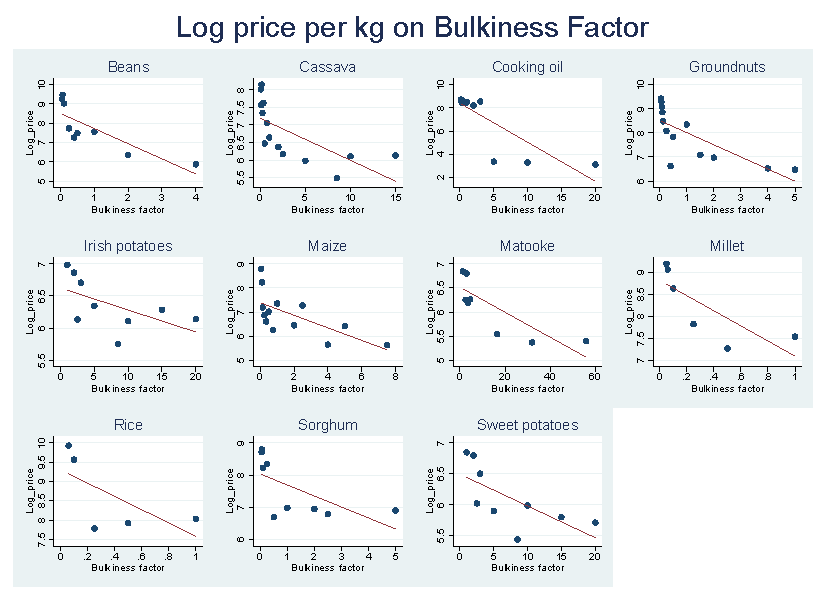
\includegraphics[frame,width=18cm, height=12cm]{Logpriceconv_linecombined.pdf}}
\caption{\textbf{Price of commodity per kg/liter on bulkiness of purchase}}
\label{fig:fig2}
\end{figure}

\hspace{1cm} Next, the idea is that savings groups encourages bulk purchasing by making you less price sensitive. I test this using the following model equation:

\boldmath
\begin{equation}
bulk purchases_{chpt} = \beta SavingsGroups_{pt}\\
+ f_c  + f_h + f_p + f_t   + \delta X_{hpt} + \epsilon_{chpt}\\
\end{equation}
\unboldmath

where $f_c$ is the fixed effect for commodity. This parameter identifies household-level preferences for good c. (for example, some household like to eat a certain crop, others don’t). 



\subsection{Results from regression analysis}\label{sec:regression2}

\hspace{1cm} In this section, I regress the bulk purchase dummy on treatment. However, I do not observe any strong association between exposure to savings groups and bulk purchases. Note that here I am not looking at if the household consumes the entire product in bulk or not; but rather I am interested in observing whether the household reports a product that was purchased in bulk units. One of the reasons why savings groups still do not result in bulk purchases could be that goods kept in bulk at home could be subject to spoilage or even theft (see \cite{aggarwal}). A further analysis requires digging into the seasonality of bulk purchases based on the commodities. In \hyperref[sec:appendix]{Appendix} Table \ref{table:bulk price}, I also regress price of commodities (in standardized units of measurement) on the bulk purchase dummy. As expected, I find a significantly negative association between the two - the bulkier the purchase, the more price discount obtained by the consumer.

\begin{table}[!h]
\centering
\begin{tabular}{llll}
 \\
& \multicolumn{3}{c}{\bfseries Bulk Purchase dummy} \\
\cline{1-4}
 {\bfseries Variables} & (1) & (2) & (3)  \\
 \hline
SavingsGroups  &  0.001 & 0.003 & 0.003 \\
 & (0.006)	& (0.006)	& (0.006) \\
 &  \\
Observations 	& 105,913 & 105,913 & 105,913  \\
R-squared  &	0.024	&	0.042		& 0.298 \\
Mean of Outcome	& 0.156	& 0.156 & 	0.156
&
Time F.E.  & YES & YES & YES \\
HH Controls & YES & YES & YES \\
Parish F.E.  & YES & YES & YES \\
HH F.E. & NO & YES & YES \\
Product F.E. & NO & NO & YES \\\hline

\cline{1-4}
\end{tabular}
\caption{\bfseries Fixed-Effects regression of bulk purchases on treatment variable}
\label{table: bulk}
\footnotesize{(Notes for table: Outcome variable represents the bulk purchase dummy which takes the value of 1 if the household reports purchasing the product in bulk units of 5 kgs and above. Note that if the household does not consume a given product in the given time period, I impute the bulk purchase dummy as 0. Column 1 represents regression with time and parish fixed effects, column 2 includes household fixed effects as well while column 3 also adds product fixed effects. The HH controls includes variables like sex of HH head, marital status and educational status of HH head, age composition brackets for household members, etc. Standard errors are clustered at the parish level in parentheses 
*** p $<$ 0.01, ** p $<$ 0.05, * p $<$ 0.1)}
\end{table}

\pagebreak
\clearpage


\section{Heterogeneity Analysis and Results}\label{sec:heterogeneity analysis and results}

\hspace{1cm} To better understand the mechanism
through which the timing of entry of savings groups influences household's welfare outcomes, I next show how treatment effects vary by characteristics of household. Here, I only look at the differential treatment effects on household's total assets and monthly earnings. Savings groups helps in significantly boosting the total value of assets both in rural and urban areas, but the effect in urban areas is almost 4 times more compared to that in rural areas. Savings groups do not seem to be significantly improving assets in female headed households, but we do a significant impact on households with male household heads. Similarly, savings groups have a significant impact on asset value of the richer households, but an insignificant impact on poor households. Finally, savings groups are seen to be much more significantly increasing household assets for households that report the primary occupation and main source of earnings to be "Farming" than for the non-farmer households. On the other hand, savings groups do not seem to be significantly improving monthly earnings for any of the heterogeneous type, however we do see a larger magnitude effect on urban households, households with female heads and non-poor, non-farmer households. One of the potential explanations for a significantly negative effect on poor households' earnings could be that savings groups help households to climb up the income ladder and migrate from poor to non-poor category. If the number of households reporting themselves to be poor declines, then average income level of poor households might decline as well. 


\begin{sidewaystable}
\centering
\begin{tabular}{lllllllll}
 \\
\cline{1-9}
\multicolumn{1}{c}{\bfseries  Variables} & \multicolumn{1}{c}{\bfseries  Rural} &  \multicolumn{1}{c}{\bfseries  Urban} & \multicolumn{1}{c}{\bfseries  Female HH head} &  \multicolumn{1}{c}{\bfseries  Male HH head} & \multicolumn{1}{c}{\bfseries  Poor} &  \multicolumn{1}{c}{\bfseries  Non-poor} & \multicolumn{1}{c}{\bfseries  Farmer} &  \multicolumn{1}{c}{\bfseries  Non-farmer}\\
\hline
SavingsGroups  & 330.938**	& 1,907.872***	& 283.197	& 690.614*** &	-306.270 &	730.717***	& 489.336** &	545.482*
 \\
 & (164.112) &	(696.833) &	(279.057)	& (250.773)	& (213.887) &	(237.768) &	(226.273) &	(328.297)
 \\
 &  \\
Observations & 7,220	& 1,974	& 3,084	& 6,259 &	1,309 & 	7,455 &	4,516 & 4,156 \\
R-squared & 0.705 &	0.801 &	0.761 &	0.786 &	0.707 &	0.773	& 0.697 &	0.814 \\
Mean of Outcome & 1854.169	& 5369.440	& 2276.686 &	2852.269	& 917.893	& 3082.054 &	1866.568 &	3488.837

&
Time F.E. & YES & YES & YES & YES & YES & YES & YES & YES \\
HH Controls & YES & YES & YES & YES & YES & YES & YES & YES  \\
Parish F.E. & YES & YES & YES & YES & YES & YES & YES & YES  \\
 HH F.E. & YES & YES & YES & YES & YES & YES & YES & YES  \\ \hline
\cline{1-9}
\end{tabular}
\caption{\bfseries Heterogeneous Fixed-Effects regression of total value of assets on treatment variable}
\label{table:heterogeneity assets}
\footnotesize{(Notes for table: In this table I investigate the heterogeneous effects of treatment on household assets by breaking down the sample of households into 8 different categories and running the regression for each one of them. The 8 categories are Rural, Urban, Poor, Non-poor, Farmer, Non-Farmer, Female-headed households and Male-headed households. I run the regressions using time, parish and household fixed effects. The HH controls includes variables like sex of HH head, marital status and educational status of HH head, age composition brackets for household members, etc. Standard errors are clustered at the parish level in parentheses 
*** p $<$ 0.01, ** p $<$ 0.05, * p $<$ 0.1)}
\end{sidewaystable}


\begin{sidewaystable}
\centering
\begin{tabular}{lllllllll}
\\
\cline{1-9}
\multicolumn{1}{c}{\bfseries  Variables} & \multicolumn{1}{c}{\bfseries  Rural} &  \multicolumn{1}{c}{\bfseries  Urban} & \multicolumn{1}{c}{\bfseries  Female HH head} &  \multicolumn{1}{c}{\bfseries  Male HH head} & \multicolumn{1}{c}{\bfseries  Poor} &  \multicolumn{1}{c}{\bfseries  Non-poor} & \multicolumn{1}{c}{\bfseries  Farmer} &  \multicolumn{1}{c}{\bfseries  Non-farmer}\\
\hline
SavingsGroups  & -0.552 &	4.644 &	3.830 &	-2.040	& -11.775***	& 2.892 &	-2.119	& 6.024 \\
 & (2.440)	& (8.334)	& (3.873)	& (2.728)	& (4.056)	& (2.916)	& (2.206) &	(5.156) \\
 &  \\
Observations & 7,232 &	1,978	& 3,093	& 6,266 &	1,313 &	7,469 &	4,519	& 4,171
 \\
R-squared & 0.612 &	0.710 &	0.653 &	0.687 &	0.630 &	0.690	& 0.532 &	0.714 \\
Mean of Outcome & 19.292	& 53.498  &	22.671 &	29.379	& 15.621	& 30.013	& 10.805	& 44.176
&
Time F.E. & YES & YES & YES & YES & YES & YES & YES & YES \\
HH Controls & YES & YES & YES & YES & YES & YES & YES & YES  \\
Parish F.E. & YES & YES & YES & YES & YES & YES & YES & YES  \\
 HH F.E. & YES & YES & YES & YES & YES & YES & YES & YES  \\ \hline
\cline{1-9}
\end{tabular}
\caption{\bfseries Heterogeneous Fixed-Effects regression of total monthly earnings on treatment variable}
\label{table:heterogeneity earnings}
\footnotesize{(Notes for table: In this table I investigate the heterogeneous effects of treatment on household total monthly earnings by breaking down the sample of households into 8 different categories and running the regression for each one of them. The 8 categories are Rural, Urban, Poor, Non-poor, Farmer, Non-Farmer, Female-headed households and Male-headed households. I run the regressions using time, parish and household fixed effects. The HH controls includes variables like sex of HH head, marital status and educational status of HH head, age composition brackets for household members, etc. Standard errors are clustered at the parish level in parentheses 
*** p $<$ 0.01, ** p $<$ 0.05, * p $<$ 0.1)}
\end{sidewaystable}


\pagebreak
\section{Robustness}\label{sec:robustness}

\hspace{1cm} It is important to note that we do not know why a community got a savings group when it gets one which could make identification of a clean model trickier. However, I make the following arguments to support exogeneity of treatment. Firstly, savings groups are set by NGOs and are supply driven- this means that presence of savings groups is not directly related to existing consumption and welfare outcomes of household nor is it related to characteristics of a community. I demonstrate this in table \ref{table:treatment charac}, where I observe that whether a savings group enters a parish or not is unrelated to how many services a parish has to offer. Similarly, it is also unrelated to whether the parish is rural or urban or small or large in terms of its population. I however, do find that most savings groups will first enter parish in urban areas and then expand on to the rural areas. In Fig \ref{fig:fig3}, I also test for parallel trends using event study graphs which show how outcome variables respond to the timing of the arrival of the savings groups. As discussed in \cite{goodman2021difference} paper, two-way fixed effects estimator is a weighted average of all possible 2x2 DD estimators that compare timing groups to each other which means some of them may have negative weights. Negative weights occur when already-treated units act as controls and changes in their treatment effects over time get subtracted from the DD estimate. This negative weighting arises when treatment effects vary over time, in which case it typically biases regression DD estimates away from the sign of the true treatment effect. To ensure that our estimates are fully robust, I also perform Goodman Bacon Decomposition of weights. As can be seen from table \ref{tab:goodman} and figure \ref{fig:fig4}, I do not encounter this issue of negative weights and the diff-in-diff estimators are pretty simiar to my TWFE estimators. Additionally, as reported earlier, the size of estimated impacts of savings groups on different household outcome measures compare with the size of estimates from RCT literature. 

\clearpage
\textbf{Event Study Plot}
\graphicspath{{Images/}}
\begin{figure}[ht]
\makebox[\textwidth][c]{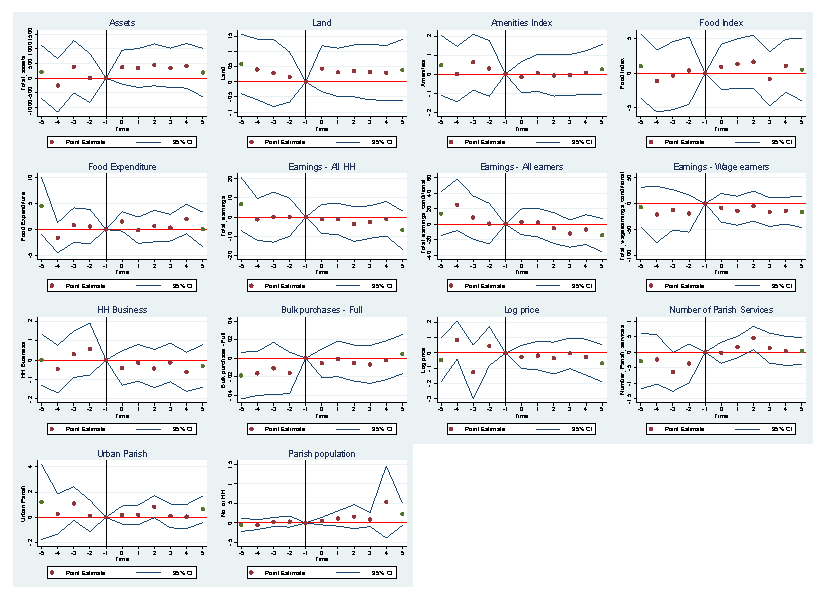
\includegraphics[frame,width=18cm, height=12cm]{eventdd_combined.pdf}}
\caption{\textbf{Event DD graphs}}
\label{fig:fig3}
\footnotesize{In this graph, I perform an event study analysis to assess how different outcome variables respond before and after treatment. The time variable stands for the difference between year of interview and year in which the parish was exposed to savings groups. All event study regressions are based on parish fixed effects with standard errors clustered at parish level except for regressions related to number of parish services, urban status of parish and number of households in parish all of which are based on district fixed effects with standard errors clustered at district level.}
\end{figure}


\clearpage
\textbf{Goodman Bacon Decomposition Plot}
\graphicspath{{Images/}}
\begin{figure}[ht]
\makebox[\textwidth][c]{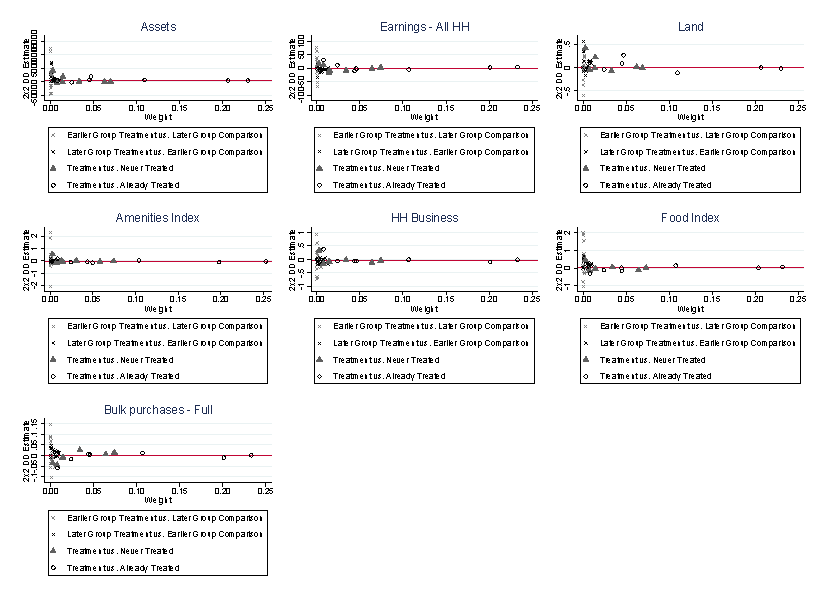
\includegraphics[frame,width=18cm, height=12cm]{ddtiming_combined.pdf}}
\caption{\textbf{Goodman Bacon Decomposition of weights}}
\label{fig:fig4}
\end{figure}


\begin{table}[htbp]
  \centering
  \csvreader[
    tabular=|c|c|c|c|c|,
    table head=\hline \textbf{Variable} & \textbf{Diff-in-Diff Estimate} & \textbf{DD Comparison} & \textbf{Weight} & \textbf{Average DD Estimate} \\\hline,
    late after line=\\\hline
  ]{Goodman_Bacon_Decomposition_Weights.csv}{}%
  {\csvcoli & \csvcolii & \csvcoliii & \csvcoliv & \csvcolv}
  \captionsetup{justification=centering}
  \caption{\bfseries Goodman Bacon Decomposition of Weights}
  \label{tab:goodman}
  \footnotesize{T: Treatment, C: Comparison}
\end{table}

\begin{table}[!h]
\centering
\begin{tabular}{lllllll}
 \\
\cline{1-7}
  & \multicolumn{3}{c} {\bfseries Savings Group in Parish} & \multicolumn{3}{c} {\bfseries Late Treatment} \\
\hline
Number of Services & 0.011*** &	-0.000	& 0.008 & 0.014*** &	0.003 &	0.004 \\
 & (0.002) &	(0.007)	& (0.005)	&  (0.002)	& (0.005)	& (0.004) \\
  & \\
Urban Parishes & -0.038	& -0.034   	& 0.010 & -0.072*	& -0.065* &	-0.097***
 \\
 & (0.056) &	(0.057)	& (0.040) & (0.041) &	(0.039)	&(0.028) \\
  & \\
Number of HH  & 0.006	& 0.006	& 0.017***	& -0.003	& -0.002	& -0.007** \\
in Parish (in 00's) & (0.011) & 	(0.01) &	(0.004) &	(0.003) &	(0.004) &	(0.003) \\
  & \\
Observations & 2,045	& 2,045 &	2,044	& 1,448
 & 	1,448 & 1,444 \\
R-squared & 0.027 &	0.041 &	0.342 & 0.076 & 0.112 & 0.433 \\
Mean of Outcome & 0.708 &	0.708 &	0.708 & 0.153 &	0.153 &	0.153
&
Time F.E. & NO & YES & YES & NO & YES & YES \\
District F.E.  & NO  & NO & YES   & NO & NO & YES\\
 \hline
\cline{1-7}
\end{tabular}
\captionsetup{justification=centering}
\caption{\bfseries Fixed-Effects regression of treatment and timing of treatment on \\ parish characteristics, parish population and rural-urban status of parish}
\label{table:treatment charac}
\footnotesize{(Notes for table: In this table I investigate if there is a selection of savings groups into parish depending on parish characteristics, urban status or parish population. The parish population is approximated by the number of households in a parish. I construct 18 dummy variables to look at 18 different services - namely - community road, government hospital, government primary school, government secondary school, private hospital, private primary  school, private secondary school, private NGO clinic, pharmacy, police station, post office, veterinary service, Agricultural extension services, markets, trunk road,  feeder road, technical school and government health center. I then add up these dummies to construct a measure for how many services are available to community members within the community. I run the regressions using no fixed effects, time fixed effects and district fixed effects. Standard errors are clustered at the district level in parentheses.
*** p $<$ 0.01, ** p $<$ 0.05, * p $<$ 0.1)}
\end{table}

\clearpage


\section{Conclusion}\label{sec:conclusion}

\hspace{1cm} Access to financial services is crucial for development, as it enhances resource mobilization needed for productive investment  and facilitates consumption smoothing. Access to savings and credit in low-income settings can improve food security as well as the ability to purchase durable assets and storable foodstuffs in bulk, even in situations where there are no improvements in income. In this paper, I studied the channel of a growing financial institution in the form of Savings groups in the context of Uganda using National Panel Survey data from 2010-2020. The period corresponded to a rapid expansion of savings groups and I employed a TWFE model that exploited the variation in the timing of arrival of a savings groups in a community. I observed that bulk quantities do trade at a discount to small quantities which means that households with savings would be less sensitive to price volatility. However, I did not find a significant evidence of increase in bulk purchases of storable foodstuffs due to exposure to savings groups. I also observed that savings groups significantly increase household’s average value of assets, however they do not have a significant impact on monthly household earnings or on household amenities. I also found a significant positive effect of savings groups on food security characterized by variety of food consumed and expenditure on food especially for households not facing any shocks during any given year.

\hspace{1cm} My results on bulk purchase behavior though insignificant is not fully without credit. It's reasonable to believe that households who save with formal or informal savings mechanisms are more likely to rely on savings in the event of an external shock, which means instead of purchasing durable foodstuffs in bulk today, households could very well be saving up money to spend on consumption and other expenses at the time of an external shock. I intend to study this aspect in my subsequent paper. 

\hspace{1cm} A number of impact evaluation studies found that the introduction of savings groups improves food security, overall consumption smoothing, livestock holding, household business outcomes and women’s empowerment ({\cite{beaman}, \cite{gash}, \cite{karlan}); however, these welfare impacts are quite muted, raising the question of why the increase in financial intermediation created by savings groups does not improve outcomes. \cite{Flynn} in their paper observe that while savings groups can help to facilitate operational expenses and cash flow thereby supporting members’ micro-enterprises – in opportunity starved contexts their transformational potential is at best limited, especially in the short run. Savings groups are known to have a profound impact on financial inclusion, economic empowerment, and social outcomes. They offer a viable alternative to traditional financial services, particularly in under-served areas. However, challenges related to management, sustainability, and scalability need to be addressed to maximize their impact. Ensuring the long-term sustainability of savings groups can be challenging, considering that while many groups are successful in the short term, maintaining their operations over time requires ongoing support and capacity-building. Besides, poor management and lack of financial literacy could also result in mismanagement or fraud. Future research should focus on strategies for overcoming these challenges and enhancing the effectiveness of savings groups.


\newpage

\printbibliography

\newpage
\section*{Appendix Tables}\label{sec:appendix}

\textbf{1. Linking Household IDs across survey years}

The UNPS survey revised the manner in which the unique HH - ID key was designed multiple times across years. Hence before performing any data cleaning and analysis operations, it is important to have consistent HH - ID keys across survey years to panelize them. For the years that UNPS updated their HH- ID keys, they also provided the old linking keys to link households across years. I first do the linking process in ascending order of time. To elaborate, I take the oldest appearing household ID key and year by year merge the updated HH - ID keys with the help of the linking keys. This gives me the updated HH-ID keys for the oldest appearing households in survey. Then I perform a reverse merge-key operation in descending order of time. This is important since there could be households that did not appear in the oldest survey period but appeared in later survey years. Thus, I want to trace these households as further back in time as possible in my data. Here, I start with the HH - ID key of households in the most recent survey year and then year by year I merge the older HH - ID keys associated with them. Finally, I get a comprehensive set of HH- ID keys which are linked across time and I give a new set of unique HH - ID keys to each household which is now consistent across survey years. In this way I use the linking HH - ID keys and create a new column of HH - IDs that are consistent across the years for each household. 

\clearpage


\textbf{ 2. Commodity breakdown}

\hspace{1cm} The consumption module provides detailed information on consumption behavior of households for 100+ commodity items that households can choose to consume from. Firstly, I combine many of these commodities into larger commodity buckets, for instance maize flour, maize cobs and maize grains will all be classified together under Maize. Then for all of these larger commodity buckets, I compute the share of expenditure on the particular commodity as a proportion of total value consumed of all commodities by a household in a given year. I drop all the commodities which have less than 1\% share in household consumption expenditure on food. Then I further, eliminate all the commodities which are perishable and therefore cannot be purchased in bulk or stored for many days. This leaves me with 11 commodity items for my analysis purpose.

\vspace{1cm}

\textbf{ 3. Conversion of Matooke prices to standardized units of measurement}


\begin{table}[htbp]
  \centering
  \csvreader[
    tabular=|c|c|c|,
    table head=\hline \textbf{Matooke} & \textbf{Number of plaintains} & \textbf{Total weight} \\\hline,
    late after line=\\\hline
  ]{Matooke_conversions.csv}{}%
  {\csvcoli & \csvcolii & \csvcoliii}
  \caption{\bfseries Price of Matooke in standardized units of measurement}
  \label{tab:matooke}
\footnotetext{Weight of a single plantain is approximately 250-300 grams}
\end{table}

\clearpage 

\textbf{ 4. Linking Community survey with household survey}

\hspace{1cm} Since community module does not have information about households, I need to use a common linking factor that links community module with household module. For the initial 2 ways, this linking factor was in the form of community codes. Thus, I could merge the two modules using community codes and link household information with savings group information. For the subsequent survey waves, I have parish codes instead as the linking factor between the two modules. Thus for subsequent waves, I use parish codes to merge the community section with the household section. 

\hspace{1cm} It is to be noted that sometimes, for the same parish name, a different code could be assigned in the survey in the later survey years. Thus for the same household belonging in the same parish, if the parish code has changed, then I create a new column of parish codes, wherein I update the parish code with the original value rather than the new value. For households that move parishes, I create another new column of parish codes wherein I retain their original parish records to link the household module with the community module, and extract savings groups information corresponding to the original parish. 

\hspace{1cm} Finally, I append all the files to get the linked community-household information across all survey years. To have as minimum missing values as possible, for the households which belong to same parish, but have missing information over the years, I make sure that parish code is still the same and then populate the preceding year information in subsequent years for these observations. In the final linked file, all households have exactly 1 unique parish associated with them which enables me to track changes in household consumption and welfare before and after the entry of savings groups into the parish. All households which belong to a given parish, will have the same savings groups information corresponding to them. Once I have the completely linked file, I create a variable which records the first year of occurrence when a savings group entered the given parish, for each parish code. This is the year when the given parish gets exposed to at least 1 savings group for the first time. If in the panel, a given parish is never exposed to any savings group, then the variable will take the value of 9999. Lastly, I create my treatment variable \textit{`SavingsGroups'} which takes the value of 1 if the year of interview is greater than or equal to the year of exposure to savings group and 0 otherwise. 

\vspace{1cm}

\textbf{ 5. Explanation of variables from household module}

\hspace{1cm}  I create 4 age bins and generate a count variable to track the number of household members who belong to each of the age bins. I obtain information on key demographic variables from the `Demographic' module of the survey data. I first use the column of `Relationship to HH head' to track the personal identifier observation corresponding to HH head. I then use that identifier to fetch the demographic information for HH head. I recode the Sex of HH head variable to be 1 if the household is headed by a Female and 0 if the household is headed by a Male. I also recode the educational status of Hh head to be 1 if the HH head has at least some level of schooling and 0 otherwise. For HH head that are married I recode the dummy to be 1 and if the HH head is single or divorced or widowed I recode the dummy to 0.

\hspace{1cm} Each survey year collects data on the primary occupation and the secondary occupation for each member of the household. It's important to note here that different members can be earning income at different frequencies (weekly/daily/monthly/hourly) and so I first standardize the frequency of payments to `Monthly'. I then add up the monthly earnings from both the primary and the secondary occupations for each household member. Finally I also add up the monthly earnings for each member to give me monthly total household earnings. I then deflate the earnings and convert it to USD and finally winsorize 5\% from each side of the tail of the distribution.

\clearpage



\clearpage

\textbf{ 6. Bulk purchase - Price Relationship}
\begin{table}[!h]
\centering
\begin{tabular}{llll}
 \\
\cline{1-4}
 {\bfseries Variables} & (1) & (2) & (3)  \\
\hline
Bulk purchase  & -2.497*** &	-2.521***	& -1.931*** \\
 & (0.038) &	(0.038) &	(0.040) \\
  &  \\
SavingsGroups & 0.015	& 0.017 & 0.034 \\
 & (0.037)	& (0.037) &	(0.037) \\
  &  \\
Bulk savings interaction & -0.045	& -0.030	& -0.084** \\
 & (0.049)	& (0.049)	& (0.040) \\
 &  \\
Observations & 49,542 &	49,537	& 49,537 \\
R-squared & 0.585	& 0.606 &	0.688 \\
Mean of Outcome & 6.774	& 6.774	& 6.774
&
Time F.E. & YES & YES & YES \\
HH Controls &  YES & YES & YES \\
Parish F.E.  & YES & YES & YES\\
HH F.E. & NO & YES & YES\\
 Product F.E. & NO & NO  & YES \\ \hline
\cline{1-5}
\end{tabular}
\caption{\bfseries Fixed-Effects regression of Price per kg in log on bulk purchases}
\footnotesize{(Notes for table: Outcome variable represents the log of price of product per kg. Column 1 represents regression with time and parish fixed effects, column 2 includes household fixed effects as well while column 3 also adds product fixed effects. The HH controls includes variables like sex of HH head, marital status and educational status of HH head, age composition brackets for household members, etc. Standard errors are clustered at the parish level in parentheses 
*** p $<$ 0.01, ** p $<$ 0.05, * p $<$ 0.1)}
\label{table:bulk price}
\end{table}

\end{document}



